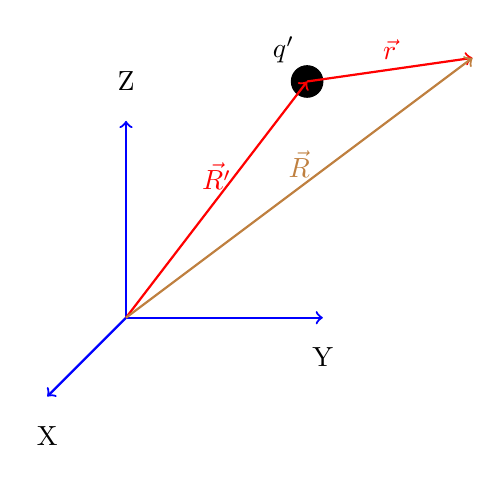
\begin{tikzpicture}
\draw [<->, blue, thick](-6.5,-4) -- (-6.5,-6.5) node (v1) {} -- (-4,-6.5);
\draw [->, blue, thick] (v1.center) -- (-7.5,-7.5);
\node at (-4,-7) {Y};
\node at (-7.5,-8) {X};
\node at (-6.5,-3.5) {Z};
\draw  [fill](-4.2,-3.5) node (v2) {} circle (0.2);
\node at (-4.5,-3.1) {$q'$};
\draw [->, red, thick] (v1.center) -- (v2.center) node [midway, above]{$\vec{R'}$};
\draw [->, red, thick] (v2.center) -- (-2.1,-3.2) node [midway, above]{$\vec{r}$};
\draw [->, brown, thick] (v1.center) -- (-2.1,-3.2) node [midway, above]{$\vec{R}$};
\end{tikzpicture}